\clearpage
\section{Appendix I: Useful Matlab Codes}
\hypertarget{code:check_grape}{The code to check all the 12-qubit GRAPE fidelities:}
\begin{lstlisting}
load Para.mat
load twpauliX_full.mat
load twpauliY_full.mat

%% Check all 90 rotations
for spin_number = 1:7
Name1 = ['twqubit_C', num2str(spin_number), '90_C_25000.txt'];
Name2 = ['twqubit_C', num2str(spin_number), '90_H_25000.txt'];
Amplitude = 25000;
Time = 1e-3;
Length = 100;
dt = Time/Length;
FirstLine = 19; % the first line which contains power and phase

Output1 = 'test1';
Output2 = 'test2';

[power1,phase1]=dataout(Name1,Output1,FirstLine,Length);
[power2,phase2]=dataout(Name2,Output2,FirstLine,Length);
%% Check
X_C = 0; Y_C = 0;
for jj = 1:7
    X_C = X_C + KIx{jj};
    Y_C = Y_C + KIy{jj};
end

X_H = 0; Y_H = 0;
for jj = 8:12
    X_H = X_H + KIx{jj};
    Y_H = Y_H + KIy{jj};
end

U = eye(2^12);
U = U*expm(-i*H*4e-6);
for ii = 1:Length
    Hext = 2*pi*(Amplitude*power1(ii)/100)*(X_C*cos(phase1(ii)/360*2*pi)-Y_C*sin(phase1(ii)/360*2*pi))+2*pi*(Amplitude*power2(ii)/100)*(X_H*cos(phase2(ii)/360*2*pi)-Y_H*sin(phase2(ii)/360*2*pi));
    U = expm(-i*(Hext+H)*dt)*U;
end
U = U*expm(-i*H*4e-6);

Utar = expm(-i*KIx{spin_number}*pi/2);

Fidelity = abs(trace(U*Utar'))/2^12

savefile = ['twqubit_C', num2str(spin_number), '90_Ufid.mat'];
save (savefile, 'U', 'Fidelity');

end
\end{lstlisting}

\clearpage
\hypertarget{code:combine_encoding1}{The code to combine GRAPE pulses into a big shape file:}
\begin{lstlisting}
%% From Z7 to Z24567
step_27 = round(1/(4*Para(2,7))/dt);
step_67_27 = round((1/(4*Para(6,7))-1/(4*Para(2,7)))/dt);
step_47_67 = round((1/(4*Para(4,7))-1/(4*Para(6,7)))/dt);
step_57_47 = round((1/(4*Para(5,7))-1/(4*Para(4,7)))/dt);
step_57 = round((1/(4*Para(5,7)))/dt);

power_encoding1_C = [power_C790_C; zeros(step_27,1);power_C2180_C; zeros(step_67_27,1); power_C6180_C; zeros(step_47_67,1);power_C4180_C; zeros(step_57_47,1);...
                                  power_C5180_C; power_C7180_C; zeros(step_57,1);power_C790_C]*Calibration/Calibration_old;
phase_encoding1_C = [phase_C790_C; zeros(step_27,1);phase_C2180_C; zeros(step_67_27,1); phase_C6180_C; zeros(step_47_67,1);phase_C4180_C; zeros(step_57_47,1);...
                                  phase_C5180_C; phase_C7180_C; zeros(step_57,1);mod((phase_C790_C+90),360)];
power_encoding1_H = [power_H790_H; zeros(step_27,1);power_H2180_H; zeros(step_67_27,1); power_H6180_H; zeros(step_47_67,1);power_H4180_H; zeros(step_57_47,1);...
                                  power_H5180_H; power_H7180_H; zeros(step_57,1);power_H790_H]*Calibration/Calibration_old;
phase_encoding1_H = [phase_H790_H; zeros(step_27,1);phase_H2180_H; zeros(step_67_27,1); phase_H6180_H; zeros(step_47_67,1);phase_H4180_H; zeros(step_57_47,1);...
                                  phase_H5180_H; phase_H7180_H; zeros(step_57,1);mod((phase_H790_H+90),360)];

total_time_encoding1 = length(power_encoding1_C)*dt;

outputfile = 'twqubit_encoding1_C';
shpfile = fopen(outputfile,'w');
    fprintf(shpfile,'##TITLE= %s\n',outputfile);
    fprintf(shpfile,'##JCAMP-DX= 5.00 Bruker JCAMP library\n');
    fprintf(shpfile,'##DATA TYPE= Shape Data\n');
    fprintf(shpfile,'##ORIGIN= Dawei''s GRAPE Pulses \n');
    fprintf(shpfile,'##OWNER= Dawei\n');
    fprintf(shpfile,'##DATE= %s\n',date);
    time = clock;
    fprintf(shpfile,'##TIME= %d:%d\n',fix(time(4)),fix(time(5)));
    fprintf(shpfile,'##MINX= %7.6e\n',min(power_encoding1_C));
    fprintf(shpfile,'##MAXX= %7.6e\n',max(power_encoding1_C));
    fprintf(shpfile,'##MINY= %7.6e\n',min(phase_encoding1_C));
    fprintf(shpfile,'##MAXY= %7.6e\n',max(phase_encoding1_C));
    fprintf(shpfile,'##$SHAPE_EXMODE= None\n');
    fprintf(shpfile,'##$SHAPE_TOTROT= %7.6e\n',90);
    fprintf(shpfile,'##$SHAPE_BWFAC= %7.6e\n',1);
    fprintf(shpfile,'##$SHAPE_INTEGFAC= %7.6e\n',1);
    fprintf(shpfile,'##$SHAPE_MODE= 1\n');
    fprintf(shpfile, '##PULSE_WIDTH= %d\n',total_time_encoding1);
    fprintf(shpfile, '##Calibration_Power= %d\n',Calibration);
    fprintf(shpfile,'##NPOINTS= %d\n',length(power_encoding1_C));
    fprintf(shpfile,'##XYPOINTS= (XY..XY)\n');

for ii = 1:length(power_encoding1_C)
    fprintf(shpfile,'  %7.6e,  %7.6e\n',power_encoding1_C(ii),phase_encoding1_C(ii));
end

    fprintf(shpfile,'##END=\n');

outputfile = 'twqubit_encoding1_H';
shpfile = fopen(outputfile,'w');
    fprintf(shpfile,'##TITLE= %s\n',outputfile);
    fprintf(shpfile,'##JCAMP-DX= 5.00 Bruker JCAMP library\n');
    fprintf(shpfile,'##DATA TYPE= Shape Data\n');
    fprintf(shpfile,'##ORIGIN= Dawei''s GRAPE Pulses \n');
    fprintf(shpfile,'##OWNER= Dawei\n');
    fprintf(shpfile,'##DATE= %s\n',date);
    time = clock;
    fprintf(shpfile,'##TIME= %d:%d\n',fix(time(4)),fix(time(5)));
    fprintf(shpfile,'##MINX= %7.6e\n',min(power_encoding1_H));
    fprintf(shpfile,'##MAXX= %7.6e\n',max(power_encoding1_H));
    fprintf(shpfile,'##MINY= %7.6e\n',min(phase_encoding1_H));
    fprintf(shpfile,'##MAXY= %7.6e\n',max(phase_encoding1_H));
    fprintf(shpfile,'##$SHAPE_EXMODE= None\n');
    fprintf(shpfile,'##$SHAPE_TOTROT= %7.6e\n',90);
    fprintf(shpfile,'##$SHAPE_BWFAC= %7.6e\n',1);
    fprintf(shpfile,'##$SHAPE_INTEGFAC= %7.6e\n',1);
    fprintf(shpfile,'##$SHAPE_MODE= 1\n');
    fprintf(shpfile, '##PULSE_WIDTH= %d\n',total_time_encoding1);
    fprintf(shpfile, '##Calibration_Power= %d\n',Calibration);
    fprintf(shpfile,'##NPOINTS= %d\n',length(power_encoding1_H));
    fprintf(shpfile,'##XYPOINTS= (XY..XY)\n');

for ii = 1:length(power_encoding1_H)
    fprintf(shpfile,'  %7.6e,  %7.6e\n',power_encoding1_H(ii),phase_encoding1_H(ii));
end

    fprintf(shpfile,'##END=\n');
\end{lstlisting}

\clearpage
\section{Appendix II: Important Figures and Experimental Spectra}
Exp 1401: Observe C7 by GRAPE as the reference. NS=10.\\
Exp 1402: Observe C2 by GRAPE as the reference. NS=10. \\

\begin{figure}[htb]
\begin{center}
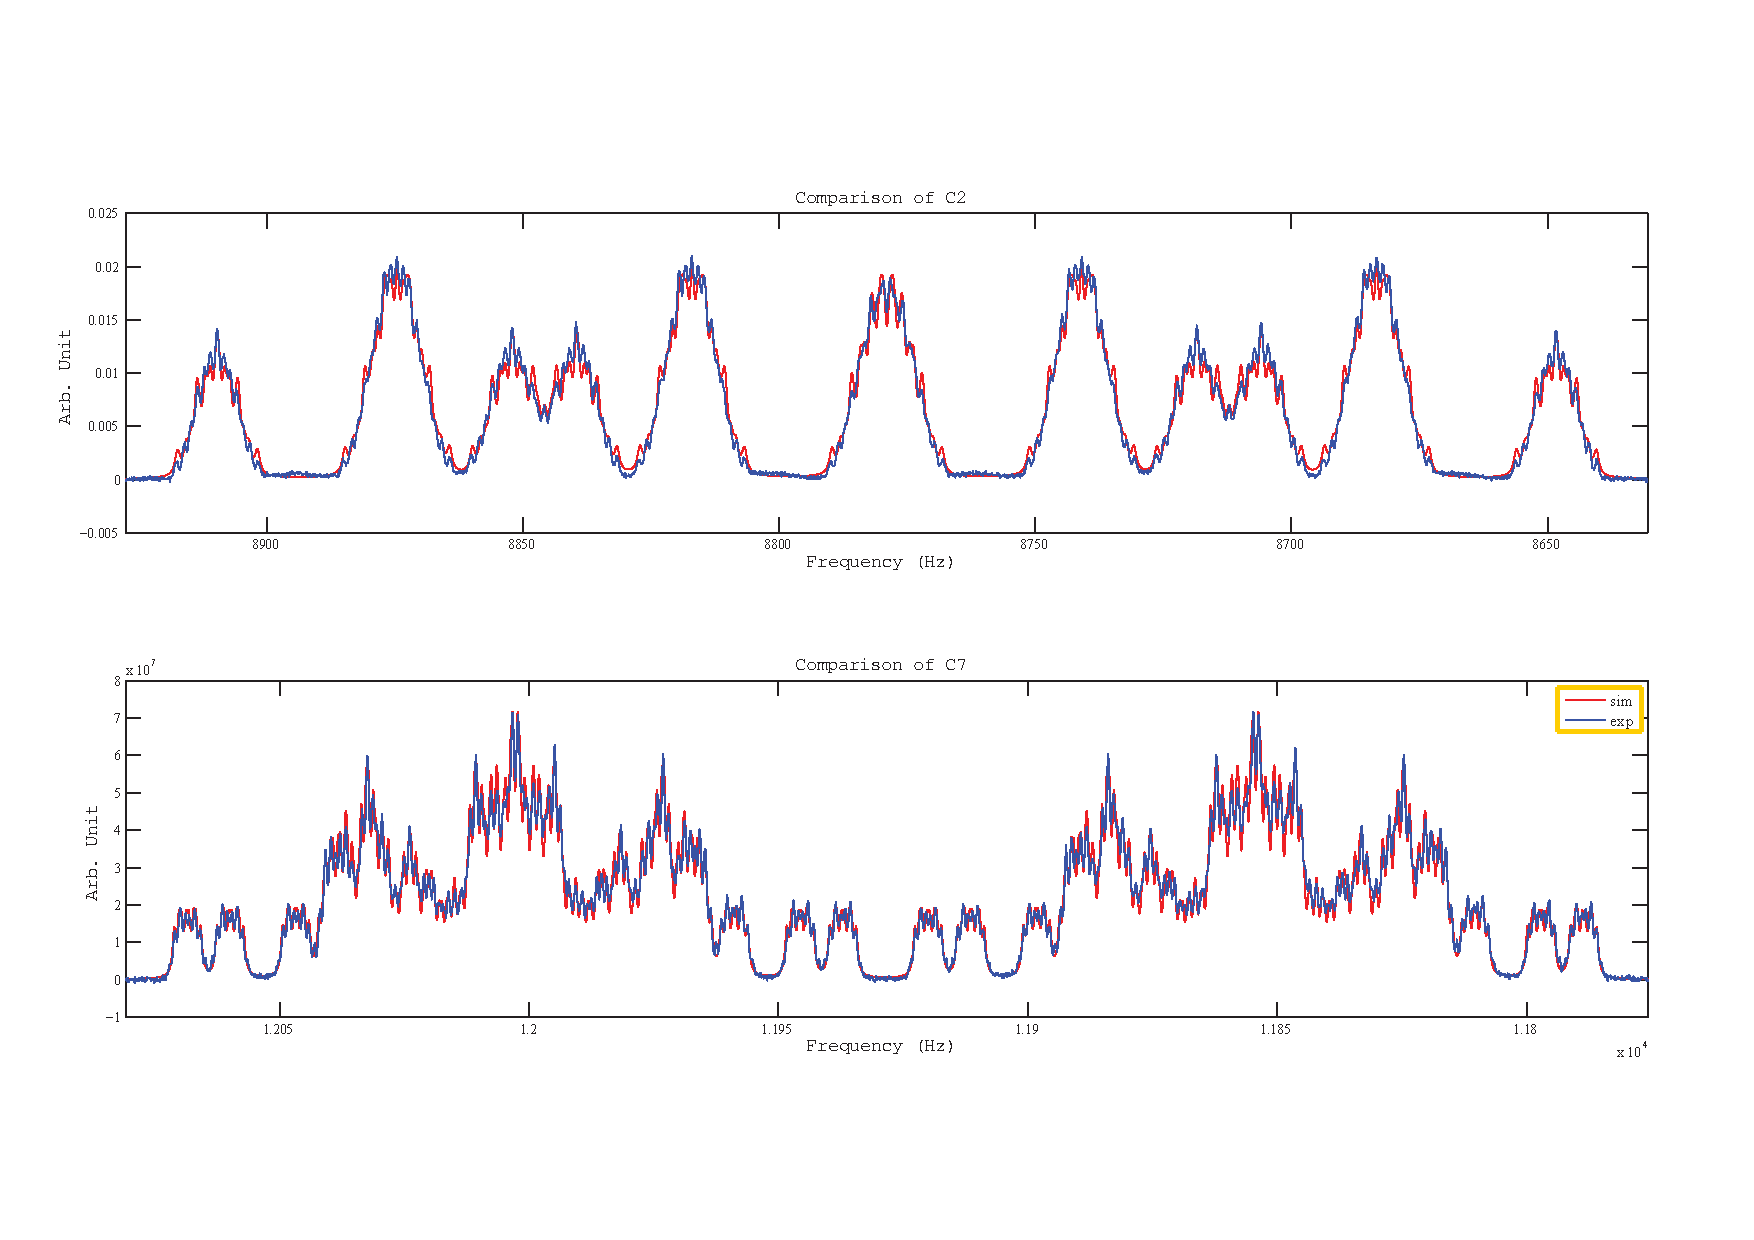
\includegraphics[width=\columnwidth]{Thermal_C2andC7.pdf}
\end{center}
\setlength{\abovecaptionskip}{-0.35cm}
\caption{\footnotesize{Comparison of the thermal for C2 and C7. Blue is experiment and Red is the simulation by the fitted Hamiltonian.}}\label{1401and1402}
\end{figure}

\clearpage
Exp 1403: Observe C7 after encoding1. NS=10.\\
Exp 1404: Observe C2 after encoding1. NS=10.\\

For C2 there is no signal because for Z24567 some couplings are close to 0 and the C2-H couplings broadens the peak. So for 12 qubits, these small couplings cannot be resolved.\\
For C7 it matches well with the simulation. However, the small couplings are annihilated due to the C7-H couplings too.

\begin{figure}[htb]
\begin{center}
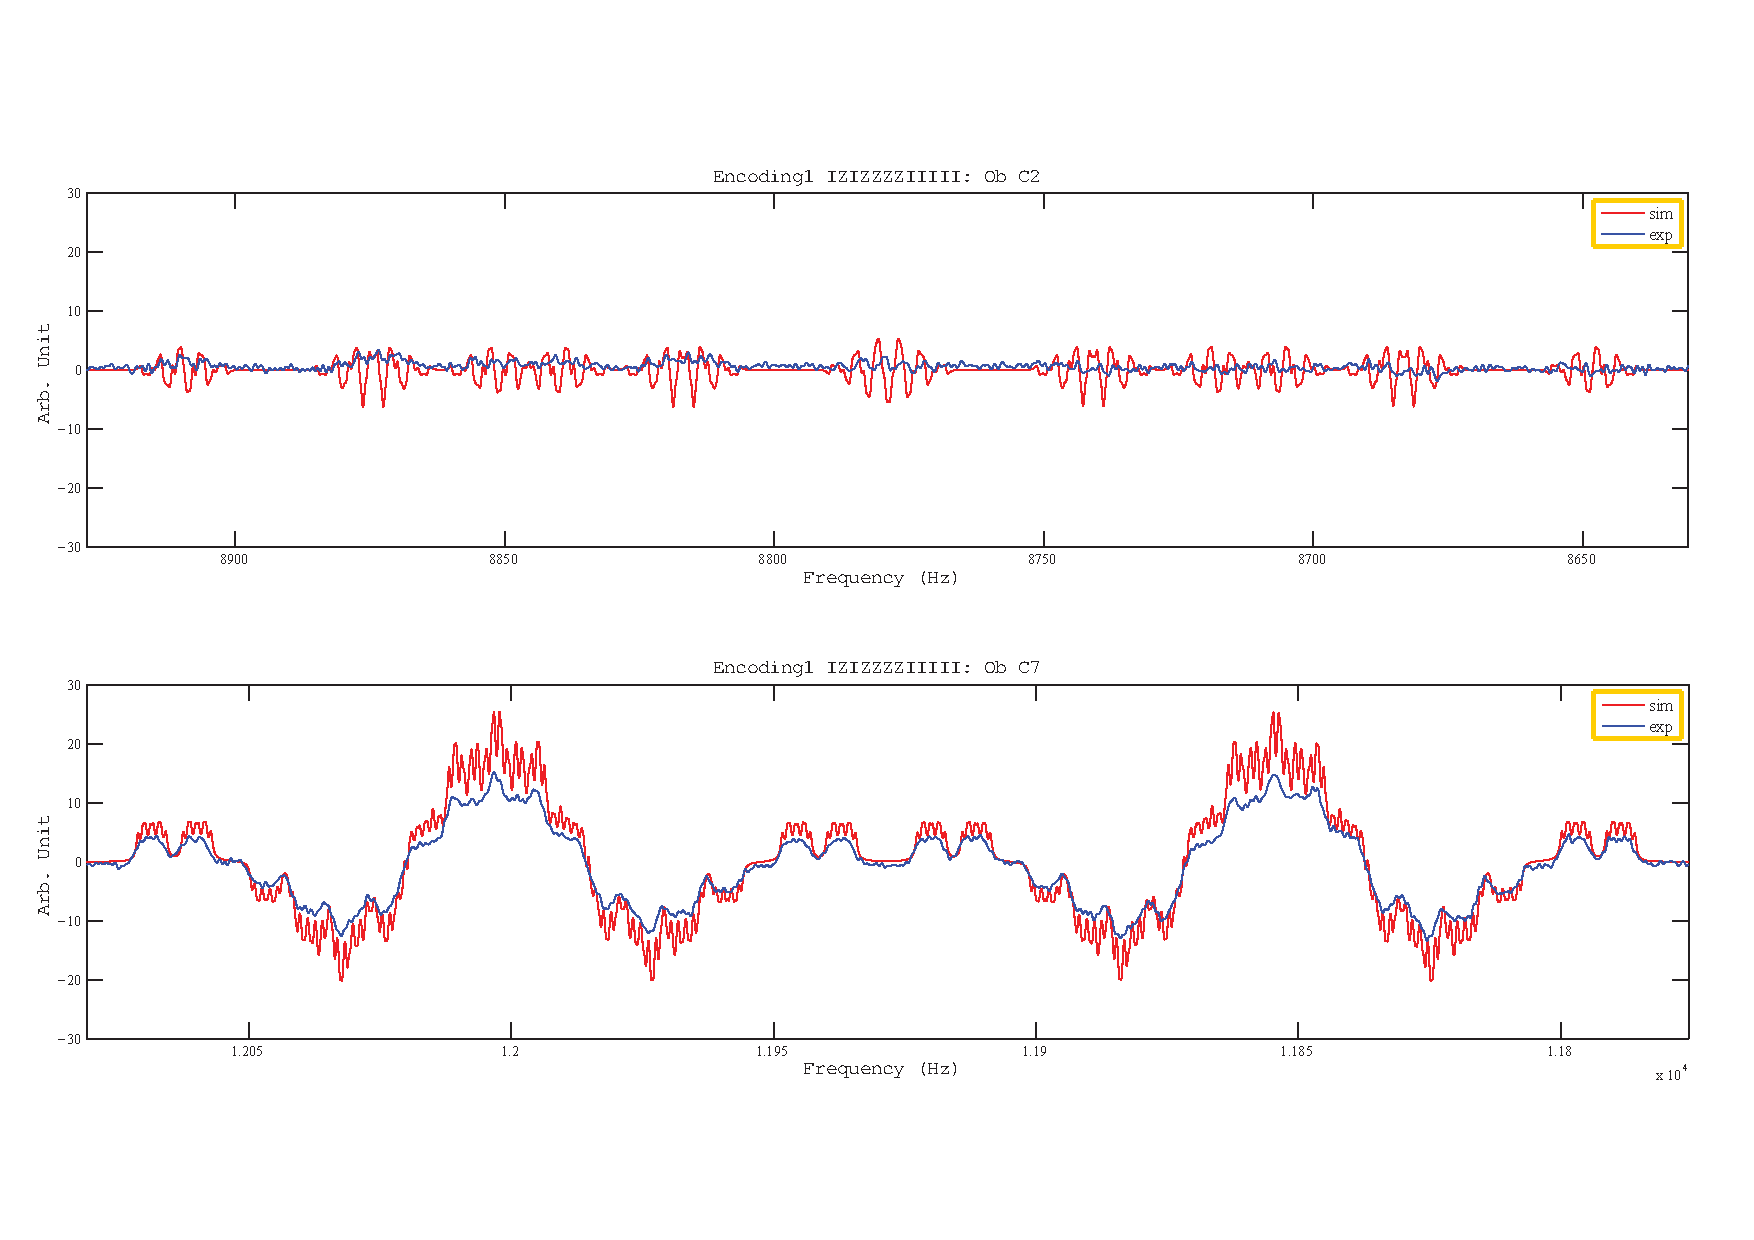
\includegraphics[width=\columnwidth]{Encoding1_without_decouple.pdf}
\end{center}
\setlength{\abovecaptionskip}{-0.35cm}
\caption{\footnotesize{Encoding 1 for C2 and C7 without H decoupled. 10 scans.}}\label{1403and1404}
\end{figure}

\clearpage
Exp 1405: Observe C7 after encoding1 and decouple H. NS=1.\\
Exp 1406: Observe C2 after encoding1 and decouple H. NS=1.\\
\textbf{Note compare with undecoupled experiments, for decoupling experiments I just used 1 scan.}

For C2 the signal is quite close to the 7-qubit case. Good.\\
For C7 the same.

\begin{figure}[htb]
\begin{center}
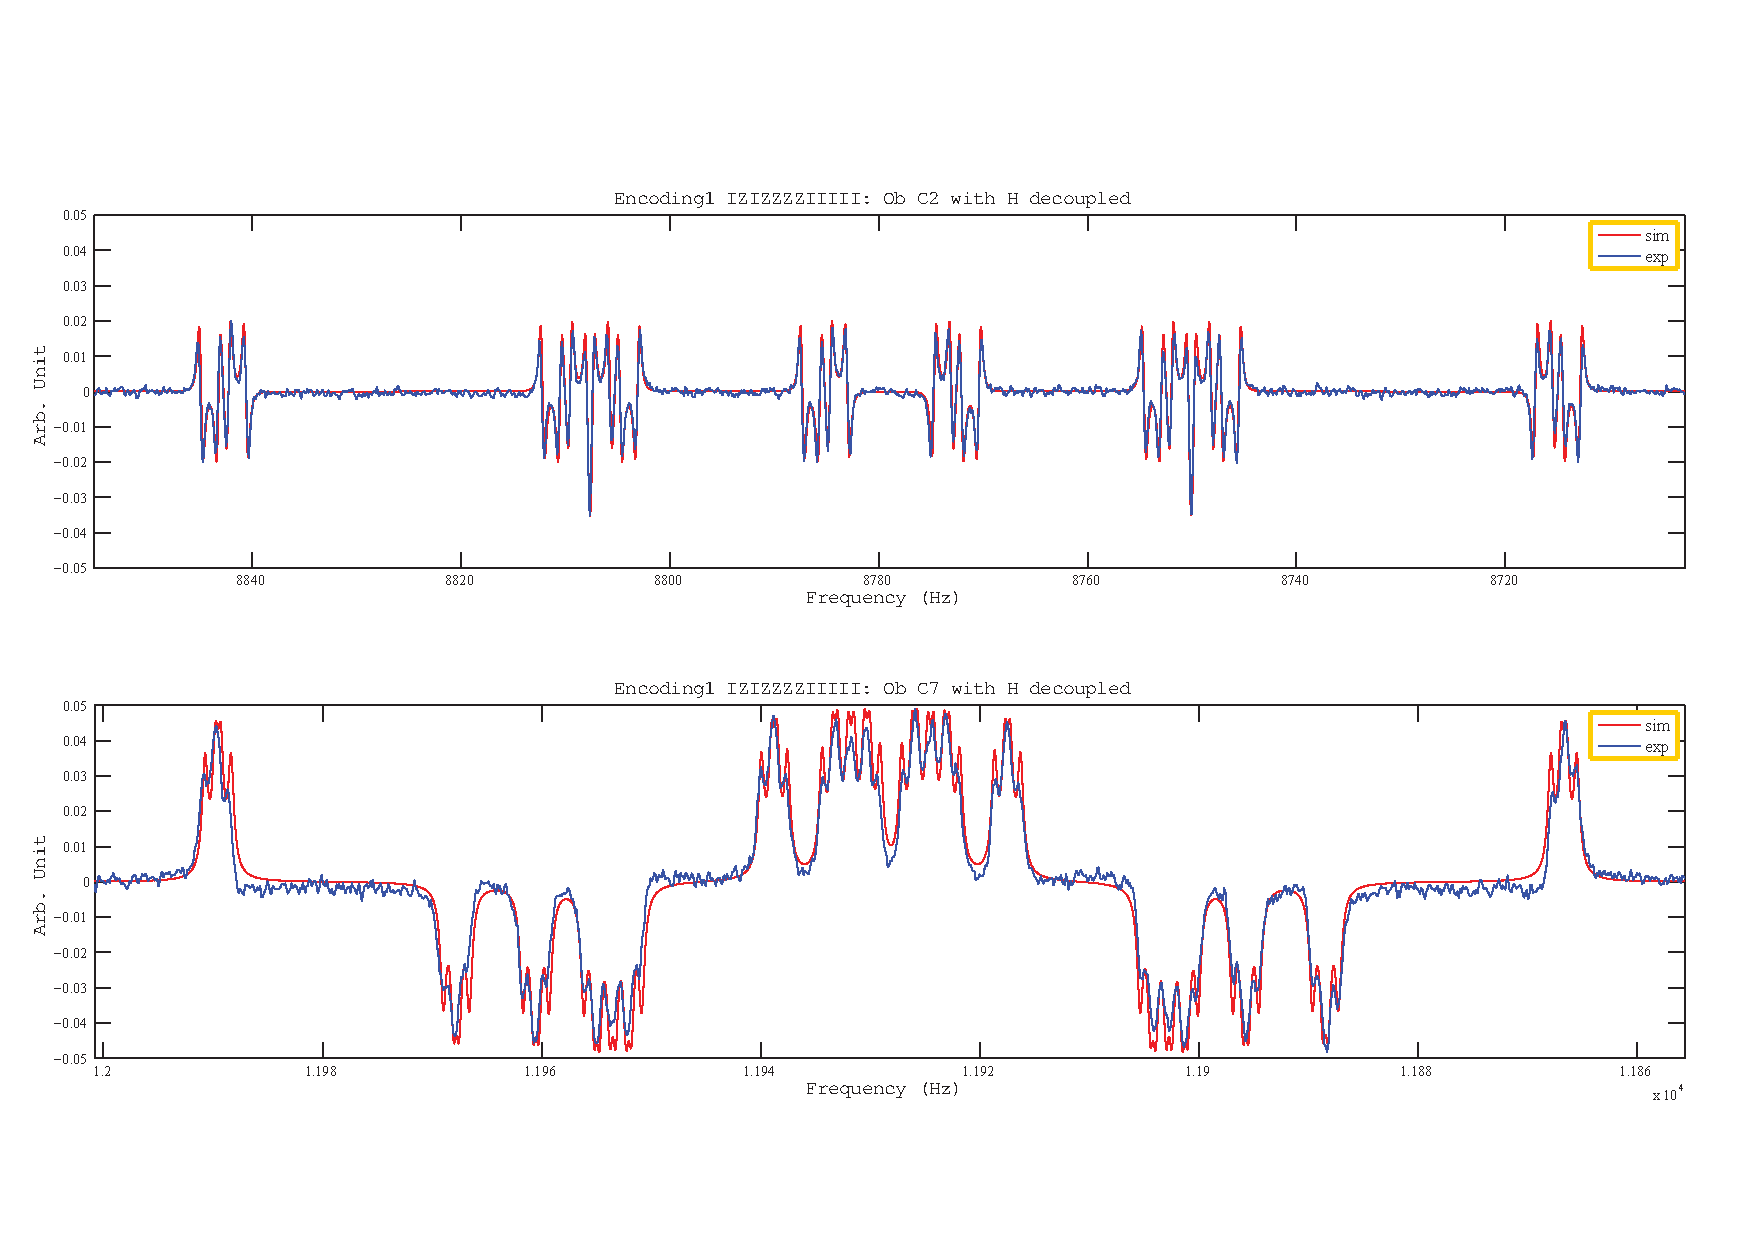
\includegraphics[width=\columnwidth]{Encoding1_with_decouple.pdf}
\end{center}
\setlength{\abovecaptionskip}{-0.35cm}
\caption{\footnotesize{Encoding 1 for C2 and C7 with H decoupled. 1 scan.}}\label{1405and1406}
\end{figure}

\clearpage
Exp 1407: Observe C7 after encoding2. NS=10.\\
Exp 1408: Observe C2 after encoding2. NS=10.\\

For C2 and C7 there are no signals due to the broaden of the C-H couplings.

\begin{figure}[htb]
\begin{center}
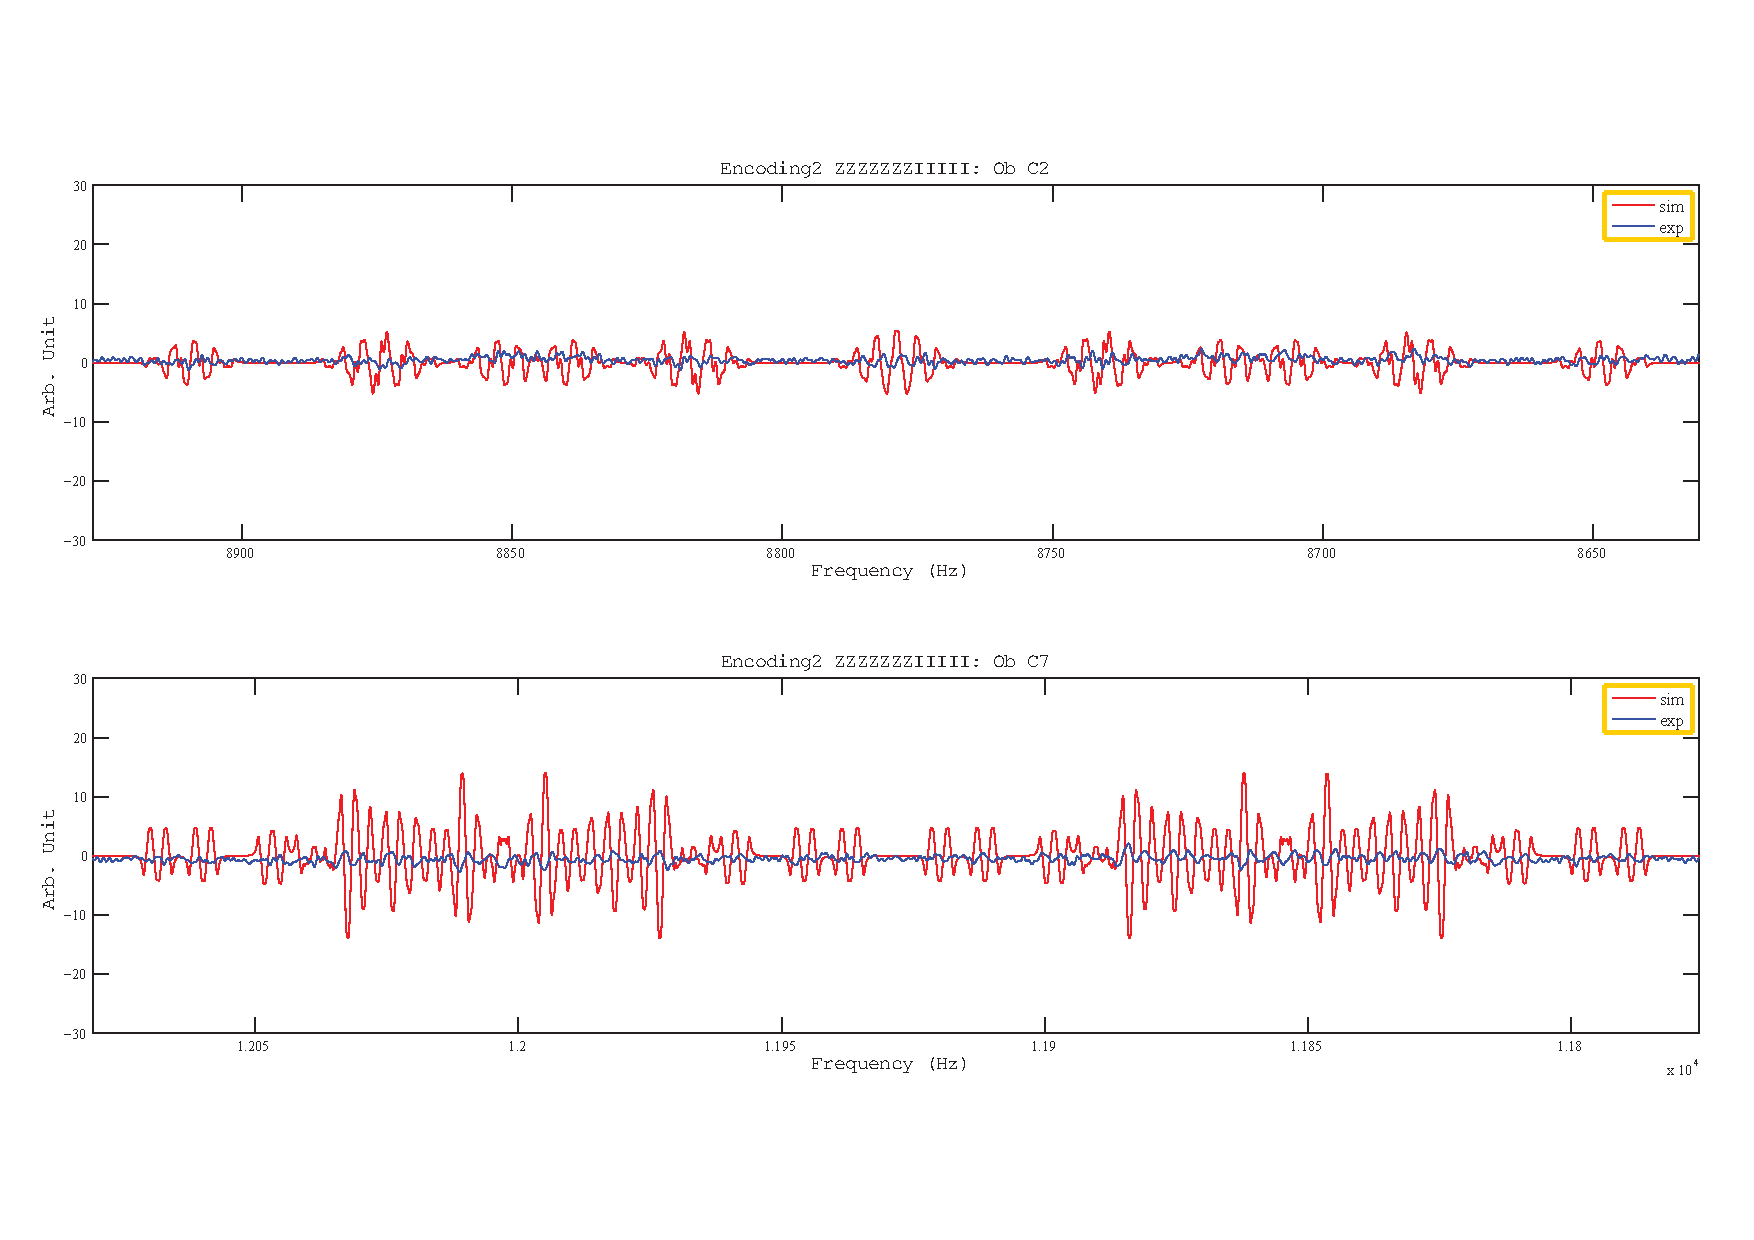
\includegraphics[width=\columnwidth]{Encoding2_without_decouple.pdf}
\end{center}
\setlength{\abovecaptionskip}{-0.35cm}
\caption{\footnotesize{Encoding 2 for C2 and C7 without H decoupled. 10 scans.}}\label{1407and1408}
\end{figure}

\clearpage
Exp 1409: Observe C7 after encoding2 and decouple H. NS=1.\\
Exp 1410: Observe C2 after encoding2 and decouple H. NS=1.\\
\textbf{Note compare with undecoupled experiments, for decoupling experiments I just used 1 scan.}

For C2 and C7 they both look nice.

\begin{figure}[htb]
\begin{center}
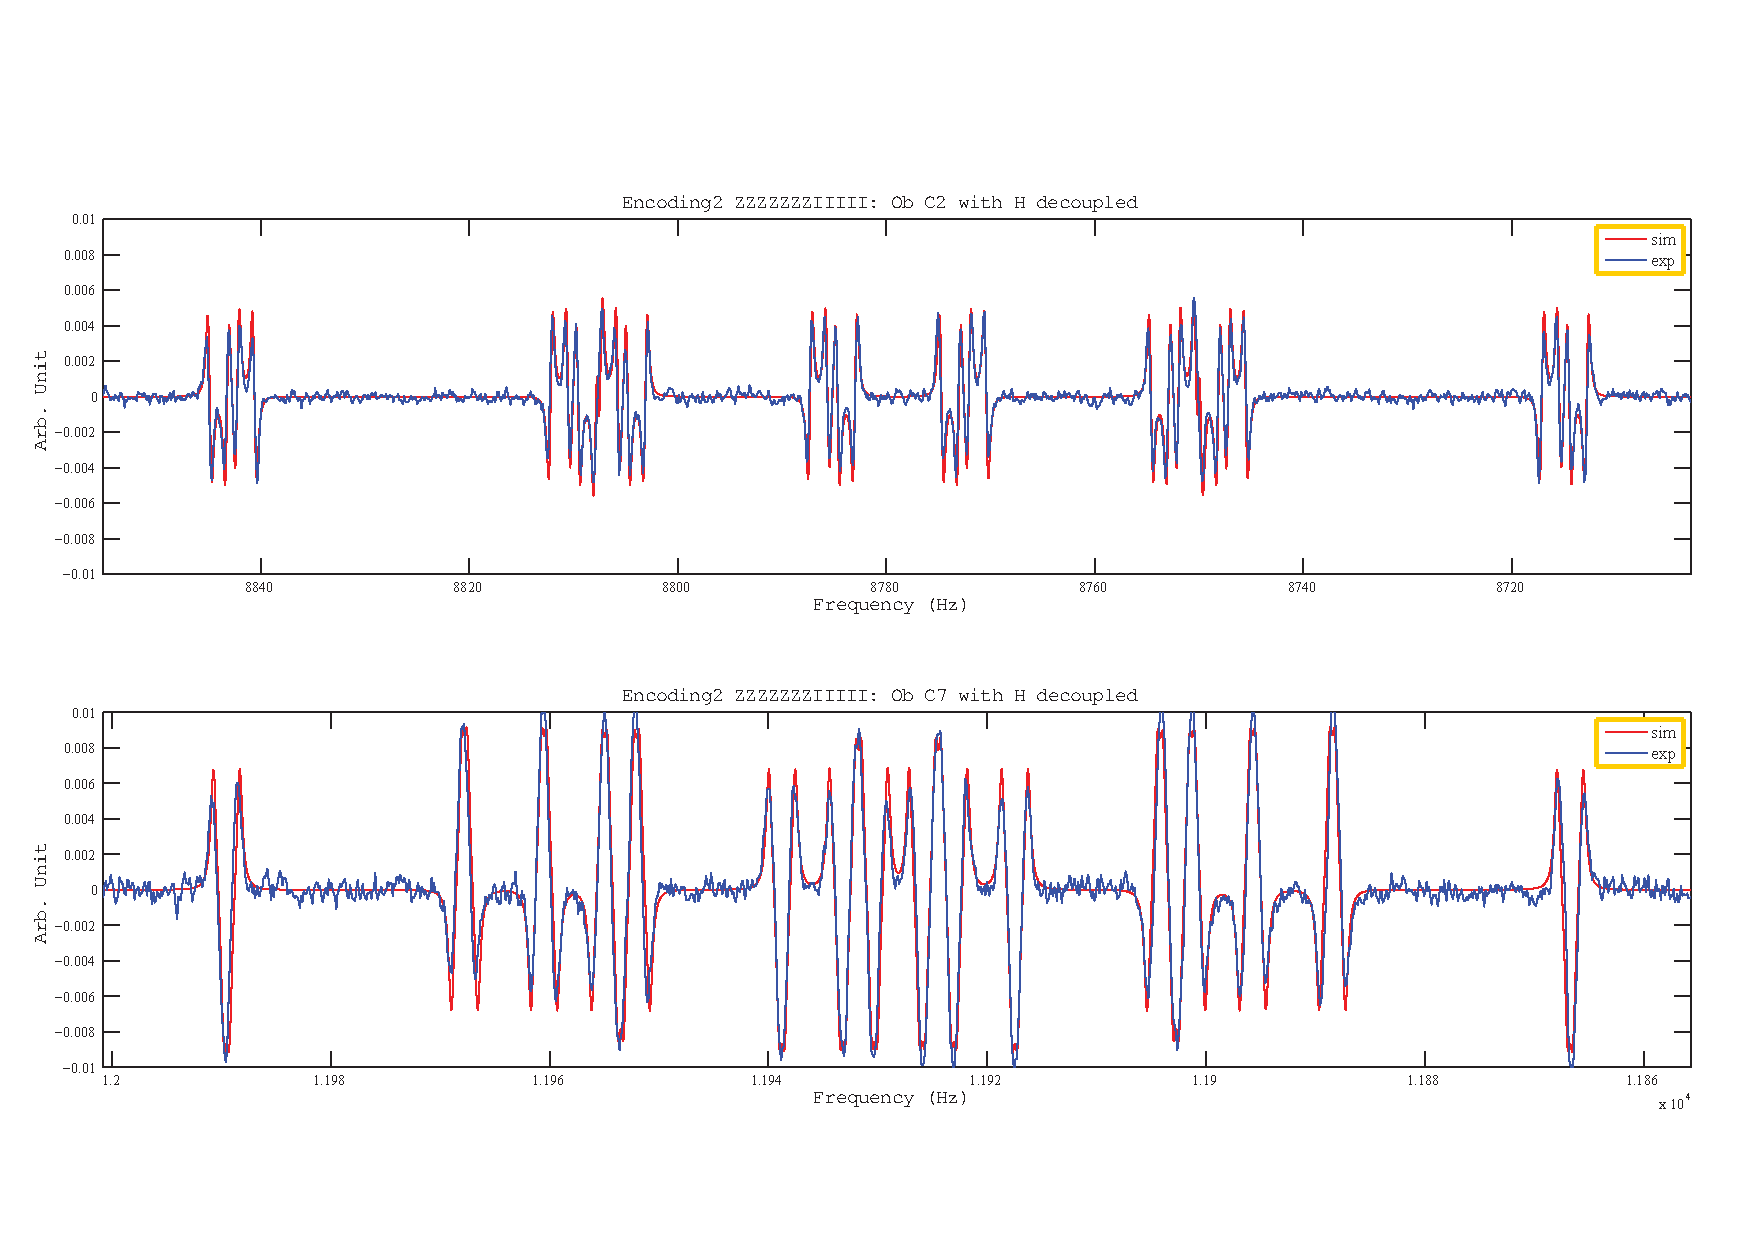
\includegraphics[width=\columnwidth]{Encoding2_with_decouple.pdf}
\end{center}
\setlength{\abovecaptionskip}{-0.35cm}
\caption{\footnotesize{Encoding 2 for C2 and C7 with H decoupled. 1 scan.}}\label{1409and1410}
\end{figure}a

\clearpage
\section{Appendix III: All Pulses for 12 qubits}

The saving folder is '\dir pulseexam\_12qubit\dir C\_rotations\dir'.

$\pi/2$ and $\pi$ rotations on every single spin.
\begin{table}[hbtp]
\begin{tabular} {c||c|c|c|c|c}
  \hline
  Rotation & Length & Fidelity & File & MaxPower C & MaxPower H\\
  \hline
  % after \\: \hline or \cline{col1-col2} \cline{col3-col4} ...
  $R_x^1(\pi/2)$ & 1ms & 0.9981 & twqubit\_C190\_Ufid.mat & 56.0\%, 14000Hz & 22.3\%, 5557Hz\\
  $R_x^2(\pi/2)$ & 1ms & 0.9986 & twqubit\_C290\_Ufid.mat & 41.7\%, 10422Hz & 23.5\%, 5878Hz\\
  $R_x^3(\pi/2)$ & 1ms & 0.9981 & twqubit\_C390\_Ufid.mat & 31.9\%, 7979.0Hz & 22.3\%, 5568Hz\\
  $R_x^4(\pi/2)$ & 1ms & 0.9976 & twqubit\_C490\_Ufid.mat & 31.6\%, 7892.0Hz & 23.8\%, 5954Hz\\
  $R_x^5(\pi/2)$ & 1ms & 0.9981 & twqubit\_C590\_Ufid.mat & 56.1\%, 14033Hz & 30.7\%, 7678Hz\\
  $R_x^6(\pi/2)$ & 1ms & 0.9979 & twqubit\_C690\_Ufid.mat & 57.3\%, 14333Hz & 34.4\%, 8595Hz\\
  $R_x^7(\pi/2)$ & 1ms & 0.9986 & twqubit\_C790\_Ufid.mat & 43.7\%, 10925Hz & 24.8\%, 6207Hz\\
  \hline
  \hline
  $R_x^1(\pi)$ & 2ms & 0.9976 & twqubit\_C1180\_Ufid.mat & 62.6\%, 15655Hz & 34.9\%, 8726Hz\\
  $R_x^2(\pi)$ & 2ms & 0.9980 & twqubit\_C2180\_Ufid.mat & 51.1\%, 12783Hz & 32.4\%, 8094Hz\\
  $R_x^3(\pi)$ & 2ms & 0.9975 & twqubit\_C3180\_Ufid.mat & 37.4\%, 9350.0Hz & 24.0\%, 5997Hz\\
  $R_x^4(\pi)$ & 2ms & 0.9970 & twqubit\_C4180\_Ufid.mat & 45.1\%, 11268Hz & 20.4\%, 5108Hz\\
  $R_x^5(\pi)$ & 2ms & 0.9975 & twqubit\_C5180\_Ufid.mat & 67.6\%, 16895Hz & 31.1\%, 7782Hz\\
  $R_x^6(\pi)$ & 2ms & 0.9976 & twqubit\_C6180\_Ufid.mat & 71.8\%, 17948Hz & 33.6\%, 8396Hz\\
  $R_x^7(\pi)$ & 2ms & 0.9977 & twqubit\_C7180\_Ufid.mat & 51.0\%, 12759Hz & 32.1\%, 8022Hz\\
  \hline
\end{tabular}
\end{table}

Pulses for the encoding part of PPS preparation.
\begin{table}[hbtp]
\begin{tabular} {c||c|c|c|c|c}
  \hline
  Rotation & Length & Fidelity & File & MaxPower C & MaxPower H\\
  \hline
  % after \\: \hline or \cline{col1-col2} \cline{col3-col4} ...
  $R_x^{5,7}(\pi)$ & 2ms & 0.9980 & twqubit\_C57180\_Ufid.mat & 32.3\%, 8072.5Hz & 24.2\%, 6049Hz\\
  $R_x^{2,3}(\pi)$ & 2ms & 0.9978 & twqubit\_C23180\_Ufid.mat & 32.4\%, 8101.5Hz & 22.8\%, 5701Hz\\
  $R_x^{2,3,4,7}(\pi/2)$ & 1ms & 0.9970 & twqubit\_C234790\_Ufid.mat & 37.4\%, 9358.3Hz & 28.9\%, 7213Hz\\
  $R_x^{1,5,6}(\pi)$ & 2ms & 0.9974 & twqubit\_C156180\_Ufid.mat & 32.2\%, 8039.7Hz & 20.3\%, 5086Hz\\
  $R_x^{2,4,7}(\pi/2)R_{-y}^{3}(\pi/2)R_{-z}^{i=2,3,4,7}((w_i-O_1)*3.36\text{ms})$ & 1ms & 0.9964 & twqubit\_C234790withPC\_Ufid.mat & 26.1\%, 6514.5Hz & 20.2\%, 5048Hz\\
  \hline
\end{tabular}
\end{table}

Pulses for polarization crush and phase cycling.
\begin{table}[hbtp]
\begin{tabular} {c||c|c|c|c|c}
  \hline
  Rotation & Length & Fidelity & File & MaxPower C & MaxPower H\\
  \hline
  % after \\: \hline or \cline{col1-col2} \cline{col3-col4} ...
  $R_x^{1-12}(\pi/2)$ & 1ms & 0.9977 & twqubit\_all90\_Ufid.mat & 27.8\%, 6956.6Hz & 30.4\%, 7594Hz\\
  $R_x^{1-6,8-12}(\pi/2)$ & 1ms & 0.9977 & twqubit\_all90butC7\_Ufid.mat & 24.5\%, 6134.9Hz & 25.0\%, 6239Hz\\
  \hline
\end{tabular}
\end{table}

Pulses for the decoding part of PPS preparation.
\begin{table}[!h]
\begin{tabular} {c||c|c|c|c|c}
  \hline
  Rotation & Length & Fidelity & File & MaxPower C & MaxPower H\\
  \hline
  % after \\: \hline or \cline{col1-col2} \cline{col3-col4} ...
  $R_x^{2,3,4,7-12}(\pi)$ & 2ms & 0.9988 & twqubit\_C2347andH180\_Ufid.mat & 61.6\%, 15400Hz & 52.2\%, 13039Hz\\
  $R_x^{1,3,4,6}(\pi/2)R_{-y}^{8-12}(\pi/2)$ & 1ms & 0.9974 & twqubit\_C134690andH90\_Ufid.mat & 24.8\%, 6203.2Hz & 22.1\%, 5529Hz\\
  $R_x^{2,3,4,5,6}(\pi)$ & 2ms & 0.9984 & twqubit\_C23456180\_Ufid.mat & 37.8\%, 9438.2Hz & 23.0\%, 5746Hz\\
  $R_{-y}^{4,6}R_{y}^{1,3}(\pi/2)R_{x}^{2}(\pi/2)R_{-z}^{1}(6.6\text{ms})$ & 1ms & 0.9982 &  twqubit\_C1234690withPC\_Ufid.mat & 28.3\%, 7070.8Hz & 26.9\%, 6717Hz\\
  $R_x^{2,7}(\pi)$ & 2ms & 0.9979 & twqubit\_C27180\_Ufid.mat & 29.1\%, 7285.3Hz & 21.7\%, 5414Hz\\
  $R_{y}^{2}(\pi/2)R_{x}^{5}(\pi/2)$ & 1ms & 0.9975 & twqubit\_C2Y5X90\_Ufid.mat & 28.9\%, 7233.9Hz & 29.2\%, 7292Hz\\
  $R_{x}^{8,9,10,11,12}(\pi/2)$ & 1ms & 0.9982 & twqubit\_H90\_Ufid.mat & 45.6\%, 11405Hz & 27.5\%, 6876Hz\\
  \hline
\end{tabular}
\end{table}

\newpage
All pulses in the saving folder '\dir pulseexam\_12qubit\dir'. The fidelities in the following table are state fidelities
\begin{table}[!h]
\begin{tabular} {c||c|c|c}
  \hline
  Files & Length & Target State & State Fidelity\\
  \hline
  % after \\: \hline or \cline{col1-col2} \cline{col3-col4} ...
  twqubit\_encoding1\_C, H & 32.98ms & IZIZZZZIIIII & 0.9831\\
  twqubit\_encoding2\_C, H & 21.28ms & ZZZZZZZIIIII & 0.9717\\
  twqubit\_encoding3\_C, H & 7.36 ms & ZZZZZZZZZZZZ & 0.9124\\
  twqubit\_phasecycling\_C, H & 1 ms & I$_{+}^{\otimes 12}$ + I$_{-}^{\otimes 12}$ & 0.9125\\
  twqubit\_decoding\_C, H & 68.96 ms & Z$_7\otimes\ket{00000000000}$ & 0.8234\\
  \hline
\end{tabular}
\end{table}

\subsection{New Pulses with 0us Buffer Delay}

Recalculated 18 pulses with 0us buffer. Here is the information.
\begin{table}[!h]
\begin{tabular} {c||c|c|c}
  \hline
  Name & Length & MaxPower C & MaxPower H\\
  \hline
  % after \\: \hline or \cline{col1-col2} \cline{col3-col4} ...
  C790 & 1ms & 46.8\%, 11697Hz & 27.9\%, 6965Hz\\
  C290 & 1ms & 37.8\%, 9456Hz & 25.8\%, 6453Hz\\
  C234790 & 1ms & 39.1\%, 9781Hz & 29.1\%, 7287Hz\\
  C234790withPC & 1ms & 25.1\%, 6286Hz & 20.5\%, 5130Hz\\
  C134690andH90 & 1ms & 27.2\%, 6803Hz & 30.3\%, 7574Hz\\
  C1234690withPC & 1ms & 28.9\%, 7226Hz & 27.3\%, 6819Hz\\
  C2Y5X90 & 1ms & 30.5\%, 7632Hz & 28.8\%, 7212Hz\\
  C590 & 1ms & 61.4\%, 15348Hz & 32.7\%, 8171Hz\\
  C2180 & 2ms & 50.9\%, 12722Hz & 31.4\%, 7859Hz\\
  C6180 & 2ms & 75.2\%, 18790Hz & 33.6\%, 8392Hz\\
  C4180 & 2ms & 47.0\%, 11760Hz & 20.7\%, 5173Hz\\
  C57180 & 2ms & 32.4\%, 8093Hz & 25.4\%, 6361Hz\\
  C1180 & 2ms & 63.0\%, 15747Hz & 35.0\%, 8744Hz\\
  C23180 & 2ms & 34.2\%, 8540Hz & 23.3\%, 5827Hz\\
  C156180 & 2ms & 31.6\%, 7899Hz & 20.7\%, 5183Hz\\
  C2347180andH180 & 2ms & 62.2\%, 15555Hz & 52.0\%, 13011Hz\\
  C23456180 & 2ms & 38.0\%, 9497Hz & 23.2\%, 5791Hz\\
  C27180 & 2ms & 28.7\%, 7176Hz & 21.5\%, 5380Hz\\
  \hline
\end{tabular}
\end{table} 